% Template for PLoS
% Version 3.5 March 2018
%
% % % % % % % % % % % % % % % % % % % % % %
%
% -- IMPORTANT NOTE
%
% This template contains comments intended
% to minimize problems and delays during our production
% process. Please follow the template instructions
% whenever possible.
%
% % % % % % % % % % % % % % % % % % % % % % %
%
% Once your paper is accepted for publication,
% PLEASE REMOVE ALL TRACKED CHANGES in this file
% and leave only the final text of your manuscript.
% PLOS recommends the use of latexdiff to track changes during review, as this will help to maintain a clean tex file.
% Visit https://www.ctan.org/pkg/latexdiff?lang=en for info or contact us at latex@plos.org.
%
%
% There are no restrictions on package use within the LaTeX files except that
% no packages listed in the template may be deleted.
%
% Please do not include colors or graphics in the text.
%
% The manuscript LaTeX source should be contained within a single file (do not use \input, \externaldocument, or similar commands).
%
% % % % % % % % % % % % % % % % % % % % % % %
%
% -- FIGURES AND TABLES
%
% Please include tables/figure captions directly after the paragraph where they are first cited in the text.
%
% DO NOT INCLUDE GRAPHICS IN YOUR MANUSCRIPT
% - Figures should be uploaded separately from your manuscript file.
% - Figures generated using LaTeX should be extracted and removed from the PDF before submission.
% - Figures containing multiple panels/subfigures must be combined into one image file before submission.
% For figure citations, please use "Fig" instead of "Figure".
% See http://journals.plos.org/plosone/s/figures for PLOS figure guidelines.
%
% Tables should be cell-based and may not contain:
% - spacing/line breaks within cells to alter layout or alignment
% - do not nest tabular environments (no tabular environments within tabular environments)
% - no graphics or colored text (cell background color/shading OK)
% See http://journals.plos.org/plosone/s/tables for table guidelines.
%
% For tables that exceed the width of the text column, use the adjustwidth environment as illustrated in the example table in text below.
%
% % % % % % % % % % % % % % % % % % % % % % % %
%
% -- EQUATIONS, MATH SYMBOLS, SUBSCRIPTS, AND SUPERSCRIPTS
%
% IMPORTANT
% Below are a few tips to help format your equations and other special characters according to our specifications. For more tips to help reduce the possibility of formatting errors during conversion, please see our LaTeX guidelines at http://journals.plos.org/plosone/s/latex
%
% For inline equations, please be sure to include all portions of an equation in the math environment.  For example, x$^2$ is incorrect; this should be formatted as $x^2$ (or $\mathrm{x}^2$ if the romanized font is desired).
%
% Do not include text that is not math in the math environment. For example, CO2 should be written as CO\textsubscript{2} instead of CO$_2$.
%
% Please add line breaks to long display equations when possible in order to fit size of the column.
%
% For inline equations, please do not include punctuation (commas, etc) within the math environment unless this is part of the equation.
%
% When adding superscript or subscripts outside of brackets/braces, please group using {}.  For example, change "[U(D,E,\gamma)]^2" to "{[U(D,E,\gamma)]}^2".
%
% Do not use \cal for caligraphic font.  Instead, use \mathcal{}
%
% % % % % % % % % % % % % % % % % % % % % % % %
%
% Please contact latex@plos.org with any questions.
%
% % % % % % % % % % % % % % % % % % % % % % % %

\documentclass[10pt,letterpaper]{article}
\usepackage[top=0.85in,left=2.75in,footskip=0.75in]{geometry}

% amsmath and amssymb packages, useful for mathematical formulas and symbols
\usepackage{amsmath,amssymb}

% Use adjustwidth environment to exceed column width (see example table in text)
\usepackage{changepage}

% Use Unicode characters when possible
\usepackage[utf8x]{inputenc}

% textcomp package and marvosym package for additional characters
\usepackage{textcomp,marvosym}

% cite package, to clean up citations in the main text. Do not remove.
\usepackage{cite}

% Use nameref to cite supporting information files (see Supporting Information section for more info)
\usepackage{nameref,hyperref}

% line numbers
\usepackage[right]{lineno}

% ligatures disabled
\usepackage{microtype}
% Helena: I have disabled because doesn't work on older latex installs and it is ugly without ligatures!
%\DisableLigatures[f]{encoding=*,family=*}

% color can be used to apply background shading to table cells only
\usepackage[table]{xcolor}

% array package and thick rules for tables
\usepackage{array}

% create "+" rule type for thick vertical lines
\newcolumntype{+}{!{\vrule width 2pt}}

% create \thickcline for thick horizontal lines of variable length
\newlength\savedwidth
\newcommand\thickcline[1]{%
  \noalign{\global\savedwidth\arrayrulewidth\global\arrayrulewidth 2pt}%
  \cline{#1}%
  \noalign{\vskip\arrayrulewidth}%
  \noalign{\global\arrayrulewidth\savedwidth}%
}

% \thickhline command for thick horizontal lines that span the table
\newcommand\thickhline{\noalign{\global\savedwidth\arrayrulewidth\global\arrayrulewidth 2pt}%
\hline
\noalign{\global\arrayrulewidth\savedwidth}}


% Remove comment for double spacing
%\usepackage{setspace}
%\doublespacing

% Text layout
\raggedright
\setlength{\parindent}{0.5cm}
\textwidth 5.25in
\textheight 8.75in

% Bold the 'Figure #' in the caption and separate it from the title/caption with a period
% Captions will be left justified
\usepackage[aboveskip=1pt,labelfont=bf,labelsep=period,justification=raggedright,singlelinecheck=off]{caption}
\renewcommand{\figurename}{Fig}

% Use the PLoS provided BiBTeX style
\bibliographystyle{plos2015}

% Remove brackets from numbering in List of References
\makeatletter
\renewcommand{\@biblabel}[1]{\quad#1.}
\makeatother



% Header and Footer with logo
\usepackage{lastpage,fancyhdr,graphicx}
\usepackage{epstopdf}
%\pagestyle{myheadings}
\pagestyle{fancy}
\fancyhf{}
%\setlength{\headheight}{27.023pt}
%\lhead{\includegraphics[width=2.0in]{PLOS-submission.eps}}
\rfoot{\thepage/\pageref{LastPage}}
\renewcommand{\headrulewidth}{0pt}
\renewcommand{\footrule}{\hrule height 2pt \vspace{2mm}}
\fancyheadoffset[L]{2.25in}
\fancyfootoffset[L]{2.25in}
\lfoot{\today}

%% Include all macros below

\newcommand{\lorem}{{\bf LOREM}}
\newcommand{\ipsum}{{\bf IPSUM}}

%% END MACROS SECTION


\begin{document}
\vspace*{0.2in}

% Title must be 250 characters or less.
\begin{flushleft}
{\Large
\textbf\newline{Galaxy for training and teaching: 2020 update} % Please use "sentence case" for title and headings (capitalize only the first word in a title (or heading), the first word in a subtitle (or subheading), and any proper nouns).
}
\newline
% Insert author names, affiliations and corresponding author email (do not include titles, positions, or degrees).
\\
Saskia Hiltemann\textsuperscript{1,2\Yinyang\textpilcrow},
Helena Rasche\textsuperscript{2\Yinyang},
AddYourNameHere\textsuperscript{3},
Bérénice Batut\textsuperscript{1\Yinyang},
with the GTN community
\\
\bigskip
\textbf{1} Clinical Bioinformatics Group, Department of Pathology, Erasmus Medical Center, Rotterdam, The Netherlands \\
\textbf{2} Affiliation Dept/Program/Center, Institution Name, City, State, Country \\
\textbf{3} Affiliation Dept/Program/Center, Institution Name, City, State, Country \\
%TODO: add your affiliation here
\bigskip

% Insert additional author notes using the symbols described below. Insert symbol callouts after author names as necessary.
%
% Remove or comment out the author notes below if they aren't used.
%
% Primary Equal Contribution Note
\Yinyang These authors contributed equally to this work.

% Additional Equal Contribution Note
% Also use this double-dagger symbol for special authorship notes, such as senior authorship.
%\ddag These authors also contributed equally to this work.

% Current address notes
%\textcurrency Current Address: Dept/Program/Center, Institution Name, City, State, Country % change symbol to "\textcurrency a" if more than one current address note
% \textcurrency b Insert second current address
% \textcurrency c Insert third current address

% Deceased author note
%\dag Deceased

% Group/Consortium Author Note
\textpilcrow Membership list can be found in the Acknowledgments section.

% Use the asterisk to denote corresponding authorship and provide email address in note below.
* saskiahiltemann@gmail.com

\end{flushleft}
% Please keep the abstract below 300 words
\section*{Abstract}In 2016, the Galaxy Training Network (GTN) developed the Galaxy Training Resource Directory (https://training.galaxyproject.org); an open, community-driven framework for the colleciton of training materials surrounding the Galaxy data analysis platform. Students and teachers alike can draw from a vast collection of tutorials on a myriad of topics. Taking advantage of the web-based Galaxy analysis framework, data analysis workflows and concepts can be learned without the need to install any software or search for example datasets. Futhermore, with the availability of serveral large public Galaxy servers supporting the training materials and offering training infrastructure as a service, this has proven to be a reliable asset to tackle the shortage of bioinformatics teaching resources, as evidenced by the increased uptake among educators.

In order to support this growing community of instructors, we have focused our efforts in recent years on adding support for teachers and trainers, for example by adding features aimed at facilitating the use of the materials in a classroom setting, simplifying the contribution flow for new materials, and adding a set of train-the-trainer materials. Here we present the latest developments in the project, for student, teachers, and systems administrators interested in training with Galaxy.



% Please keep the Author Summary between 150 and 200 words
% Use first person. PLOS ONE authors please skip this step.
% Author Summary not valid for PLOS ONE submissions.
\section*{Author summary}
Lorem ipsum dolor sit amet, consectetur adipiscing elit. Curabitur eget porta erat. Morbi consectetur est vel gravida pretium. Suspendisse ut dui eu ante cursus gravida non sed sem. Nullam sapien tellus, commodo id velit id, eleifend volutpat quam. Phasellus mauris velit, dapibus finibus elementum vel, pulvinar non tellus. Nunc pellentesque pretium diam, quis maximus dolor faucibus id. Nunc convallis sodales ante, ut ullamcorper est egestas vitae. Nam sit amet enim ultrices, ultrices elit pulvinar, volutpat risus.

%\linenumbers

% Use "Eq" instead of "Equation" for equation citations.
\section*{Introduction}
Lorem ipsum dolor sit~\cite{bib1} amet, consectetur adipiscing elit. Curabitur eget porta erat. Morbi consectetur est vel gravida pretium. Suspendisse ut dui eu ante cursus gravida non sed sem. Nullam Eq~(\ref{eq:schemeP}) sapien tellus, commodo id velit id, eleifend volutpat quam. Phasellus mauris velit, dapibus finibus elementum vel, pulvinar non tellus. Nunc pellentesque pretium diam, quis maximus dolor faucibus id.~\cite{bib2} Nunc convallis sodales ante, ut ullamcorper est egestas vitae. Nam sit amet enim ultrices, ultrices elit pulvinar, volutpat risus.

\begin{eqnarray}
\label{eq:schemeP}
	\mathrm{P_Y} = \underbrace{H(Y_n) - H(Y_n|\mathbf{V}^{Y}_{n})}_{S_Y} + \underbrace{H(Y_n|\mathbf{V}^{Y}_{n})- H(Y_n|\mathbf{V}^{X,Y}_{n})}_{T_{X\rightarrow Y}},
\end{eqnarray}

\section*{Materials and methods}
\subsection*{Etiam eget sapien nibh}

% For figure citations, please use "Fig" instead of "Figure".
Nulla mi mi, Fig~\ref{fig1} venenatis sed ipsum varius, volutpat euismod diam. Proin rutrum vel massa non gravida. Quisque tempor sem et dignissim rutrum. Lorem ipsum dolor sit amet, consectetur adipiscing elit. Morbi at justo vitae nulla elementum commodo eu id massa. In vitae diam ac augue semper tincidunt eu ut eros. Fusce fringilla erat porttitor lectus cursus, \nameref{S1_Video} vel sagittis arcu lobortis. Aliquam in enim semper, aliquam massa id, cursus neque. Praesent faucibus semper libero.

% Place figure captions after the first paragraph in which they are cited.
\begin{figure}[!h]
\caption{{\bf Bold the figure title.}
Figure caption text here, please use this space for the figure panel descriptions instead of using subfigure commands. A: Lorem ipsum dolor sit amet. B: Consectetur adipiscing elit.}
\label{fig1}
\end{figure}

% Results and Discussion can be combined.
\section*{Results}
Nulla mi mi, venenatis sed ipsum varius, Table~\ref{table1} volutpat euismod diam. Proin rutrum vel massa non gravida. Quisque tempor sem et dignissim rutrum. Lorem ipsum dolor sit amet, consectetur adipiscing elit. Morbi at justo vitae nulla elementum commodo eu id massa. In vitae diam ac augue semper tincidunt eu ut eros. Fusce fringilla erat porttitor lectus cursus, vel sagittis arcu lobortis. Aliquam in enim semper, aliquam massa id, cursus neque. Praesent faucibus semper libero.

% Place tables after the first paragraph in which they are cited.
\begin{table}[!ht]
\begin{adjustwidth}{-2.25in}{0in} % Comment out/remove adjustwidth environment if table fits in text column.
\centering
\caption{
{\bf Table caption Nulla mi mi, venenatis sed ipsum varius, volutpat euismod diam.}}
\begin{tabular}{|l+l|l|l|l|l|l|l|}
\hline
\multicolumn{4}{|l|}{\bf Heading1} & \multicolumn{4}{|l|}{\bf Heading2}\\ \thickhline
$cell1 row1$ & cell2 row 1 & cell3 row 1 & cell4 row 1 & cell5 row 1 & cell6 row 1 & cell7 row 1 & cell8 row 1\\ \hline
$cell1 row2$ & cell2 row 2 & cell3 row 2 & cell4 row 2 & cell5 row 2 & cell6 row 2 & cell7 row 2 & cell8 row 2\\ \hline
$cell1 row3$ & cell2 row 3 & cell3 row 3 & cell4 row 3 & cell5 row 3 & cell6 row 3 & cell7 row 3 & cell8 row 3\\ \hline
\end{tabular}
\begin{flushleft} Table notes Phasellus venenatis, tortor nec vestibulum mattis, massa tortor interdum felis, nec pellentesque metus tortor nec nisl. Ut ornare mauris tellus, vel dapibus arcu suscipit sed.
\end{flushleft}
\label{table1}
\end{adjustwidth}
\end{table}


%PLOS does not support heading levels beyond the 3rd (no 4th level headings).
\subsection*{\lorem\ and \ipsum\ nunc blandit a tortor}
\subsubsection*{3rd level heading}
Maecenas convallis mauris sit amet sem ultrices gravida. Etiam eget sapien nibh. Sed ac ipsum eget enim egestas ullamcorper nec euismod ligula. Curabitur fringilla pulvinar lectus consectetur pellentesque. Quisque augue sem, tincidunt sit amet feugiat eget, ullamcorper sed velit. Sed non aliquet felis. Lorem ipsum dolor sit amet, consectetur adipiscing elit. Mauris commodo justo ac dui pretium imperdiet. Sed suscipit iaculis mi at feugiat.

\begin{enumerate}
	\item{react}
	\item{diffuse free particles}
	\item{increment time by dt and go to 1}
\end{enumerate}


\subsection*{Sed ac quam id nisi malesuada congue}

Nulla mi mi, venenatis sed ipsum varius, volutpat euismod diam. Proin rutrum vel massa non gravida. Quisque tempor sem et dignissim rutrum. Lorem ipsum dolor sit amet, consectetur adipiscing elit. Morbi at justo vitae nulla elementum commodo eu id massa. In vitae diam ac augue semper tincidunt eu ut eros. Fusce fringilla erat porttitor lectus cursus, vel sagittis arcu lobortis. Aliquam in enim semper, aliquam massa id, cursus neque. Praesent faucibus semper libero.

\begin{itemize}
	\item First bulleted item.
	\item Second bulleted item.
	\item Third bulleted item.
\end{itemize}

\section*{Discussion}
Nulla mi mi, venenatis sed ipsum varius, Table~\ref{table1} volutpat euismod diam. Proin rutrum vel massa non gravida. Quisque tempor sem et dignissim rutrum. Lorem ipsum dolor sit amet, consectetur adipiscing elit. Morbi at justo vitae nulla elementum commodo eu id massa. In vitae diam ac augue semper tincidunt eu ut eros. Fusce fringilla erat porttitor lectus cursus, vel sagittis arcu lobortis. Aliquam in enim semper, aliquam massa id, cursus neque. Praesent faucibus semper libero~\cite{bib3}.

\section*{Conclusion}

CO\textsubscript{2} Maecenas convallis mauris sit amet sem ultrices gravida. Etiam eget sapien nibh. Sed ac ipsum eget enim egestas ullamcorper nec euismod ligula. Curabitur fringilla pulvinar lectus consectetur pellentesque. Quisque augue sem, tincidunt sit amet feugiat eget, ullamcorper sed velit.

Sed non aliquet felis. Lorem ipsum dolor sit amet, consectetur adipiscing elit. Mauris commodo justo ac dui pretium imperdiet. Sed suscipit iaculis mi at feugiat. Ut neque ipsum, luctus id lacus ut, laoreet scelerisque urna. Phasellus venenatis, tortor nec vestibulum mattis, massa tortor interdum felis, nec pellentesque metus tortor nec nisl. Ut ornare mauris tellus, vel dapibus arcu suscipit sed. Nam condimentum sem eget mollis euismod. Nullam dui urna, gravida venenatis dui et, tincidunt sodales ex. Nunc est dui, sodales sed mauris nec, auctor sagittis leo. Aliquam tincidunt, ex in facilisis elementum, libero lectus luctus est, non vulputate nisl augue at dolor. For more information, see \nameref{S1_Appendix}.





% TABLES, todo: move.
\begin{table}[]
	\centering
	\caption{Implementation of the ``10 simple rules for making training materials FAIR'' in the training material\label{tbl:rulesforfair}}
	\begin{tabular}{p{0.5\textwidth}p{0.5\textwidth}}
		Rules                                                                                            & Implementation in the training material\\\hline
		Plan to share your training materials online                                                     & Online training material portfolio, managed via a GitHub repository and pull requests to submit tutorials\\
		Improve findability of your training materials by properly describing them                       & Rich metadata associated with each tutorial that are visible and accessible via schemas on each tutorial webpage\\
		Give your training materials a unique identity                                                   & URL persistency with redirection in case of renaming of tutorials\\
		Data used for tutorials stored on Zenodo  and associated with a Digital Object Identifiers (DOI) & Register your training materials online\\
		Automatically registered on the ELIXIR's Training e-Support System, TeSS                         & If appropriate, define access rules for your training materials\\
		Online and free to use                                                                           & Use an interoperable format for your training materials\\
		Content of the tutorials and slides written in Markdown                                          & Metadata associated with tutorials in YAML, Workflows stored in JSON\\
		Make your training materials (re)usable for trainers                                             & Online. Rich metadata associated with each tutorial: title, contributor details, license, description, learning outcomes, audience, requirements, tags/keywords, duration, date of last revision. Strong technical support for each tutorial: workflow, data on Zenodo and also available as data libraries on usegalaxy.*, tools installable via the Galaxy Tool Shed, list of possible Galaxy instances with the needed tools.\\
		Make your training materials (re)usable for trainees                                             & Online and easy to follow hands-on tutorials. Rich metadata with ``Specific, Measurable, Attainable, Realistic and Time bound'' (SMART) learning outcomes following the Bloom's taxonomy. Requirements and follow-up tutorials to build learning parth. Provide list of Galaxy instances offering needed tools, data on Zenodo and also available as data libraries on usegalaxy.*\\
		Make your training materials contribution friendly and citable                                   & Open and collaborative infrastructure with contribution guidelines, a CONTRIBUTION file and a chat. Details to cite tutorials and give credit to contributors available at the end of each tutorial.\\
		Keep your training materials up-to-date                                                          & Open, collaborative and transparent peer-review and curation process. Short time between updates (Table …)\\
	\end{tabular}
\end{table}

\begin{table}[]
	\centering
	\caption{Top 10 tutorials in terms of filled embedded feedback form. Table extracted using \href{https://github.com/bebatut/galaxy-training-material-stats/blob/master/src/extract_repo_content_stats.ipynb}{Jupyter Notebook} on 2019-04-12\label{tbl:toptentutorials}}
	\begin{tabular}{p{0.8\textwidth}p{0.15\textwidth}}
		Tutorial                                                             & Number of responses \\\hline
		A short introduction to Galaxy (Introduction)                        & 174 \\
		Galaxy 101 (Introduction)                                            & 80 \\
		Quality Control (Sequence analysis)                                  & 73 \\
		Reference-based RNA-Seq data analysis (Transcriptomics)              & 56 \\
		From peaks to genes (Introduction)                                   & 44 \\
		Visualization of RNA-Seq results with Volcano Plot (Transcriptomics) & 20 \\
		Mapping (Sequence analysis)                                          & 19 \\
		NGS data logistics (Introduction)                                    & 19 \\
		16S Microbial Analysis with mothur (extended) (Metagenomics)         & 16 \\
		RNA-Seq reads to counts (Transcriptomics)                            & 14
	\end{tabular}
\end{table}


\begin{table}[]
	\centering
	\caption{Implementation of the ``Ten simple rules for collaborative lesson development''\cite{Devenyi_2018} in the training material\label{tbl:tensimplerules}}
	\begin{tabular}{p{0.5\textwidth}p{0.5\textwidth}}
		Rules & Implementation in the training material \\
		Clarify audience & Tutorial metadata includes level indicators (introductory, intermediate, advanced) and a list of prerequisite tutorials as recommended prior knowledge. This information is rendered at the top of each tutorial. \\
		Make lessons modular & Learning paths \\
		Teach best practice lesson development & In order to support the community of training developers, a ``Contributing'' topic was created containing 10 tutorials describing how to create new content. Furthermore, quarterly online collaboration fest(CoFests) are organized, where contributors can get direct support  \\
		Encourage and empower contributors & Involve them in reviews. Mentor them. Encourage them to become maintainers. Planemo \\
		Build community around lessons & CoFests and Community calls. Chat \\
		Publish periodically and recognize contributions & Author list on tutorials. Hall of fame. Citation at the end of the tutorial. Tweet about new or updated tutorials. List of new or updated tutorials in community newsletter. Soon: publication of tutorials via article \\
		Evaluate lessons at several scales & PR review, Trainee feedback, Instructor feedback, Workflow testing \\
		Reduce, re-use, recycle & Snippets. Share content between tutorials. Small modular tutorials linked with learning paths \\
		Link to other resources & Citations. Gallantries? \\
		You can't please everyone & but we can try (several different Galaxy introduction tutorials). Aim to clearly state what the tutorial does and does not cover, at the start.  \\
	\end{tabular}
\end{table}

\begin{figure}[!ht]
	\centering
	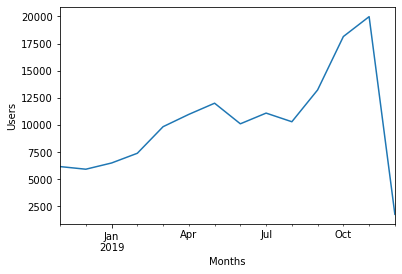
\includegraphics[width=\textwidth]{images/visits-per-month.png}
	\caption{Number of visits per month on http://training.galaxyproject.org/ given the Google Analytics stats.\label{fig:visits}}
\end{figure}

\begin{figure}[!ht]
	\centering
	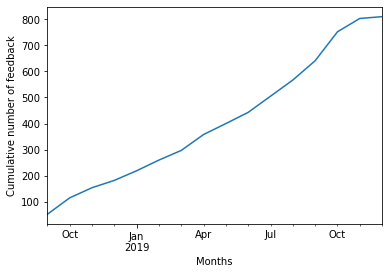
\includegraphics[width=0.45\textwidth]{images/feedback.png}
	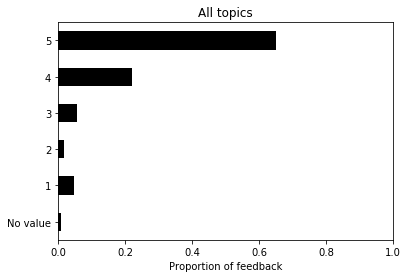
\includegraphics[width=0.45\textwidth]{images/feedback-scores.png}
	\caption{Number and results of the embedded feedback in the tutorials. 3 questions are asked in the form: ``How much did you like this tutorial?'' (from 1 to z5), ``What did you like?``, ``What could be improved?''.\label{fig:feedback}}
\end{figure}

\begin{figure}[!ht]
	\centering
	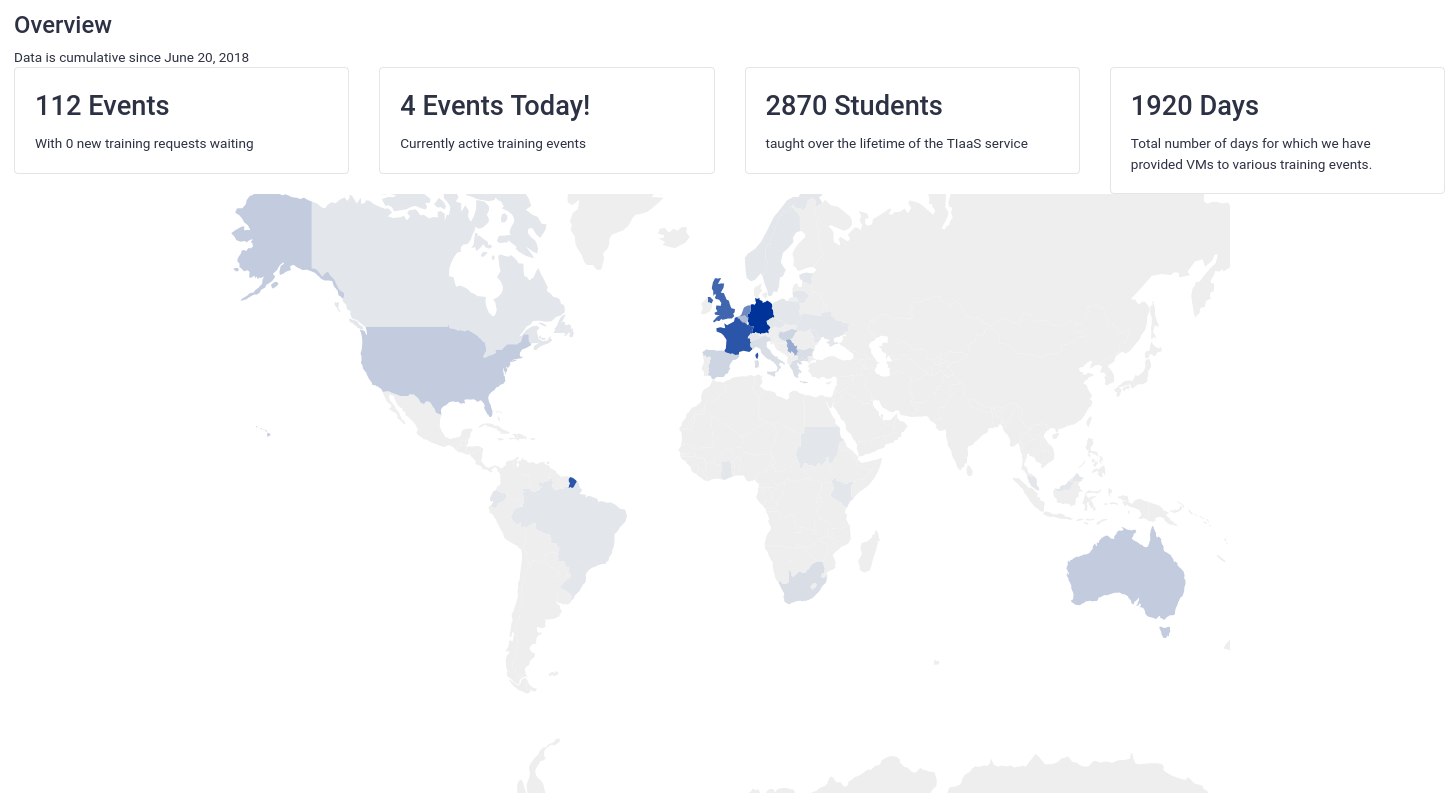
\includegraphics[width=0.8\textwidth]{images/tiaas-map.png}
	\caption{This setup has scaled well with administration time and cost, since June 2018 Galaxy Europe has hosted 66 trainings with over 2800 students with minimal overhead.\label{fig:tiaas-map}}
\end{figure}

\begin{figure}[!ht]
	\centering
	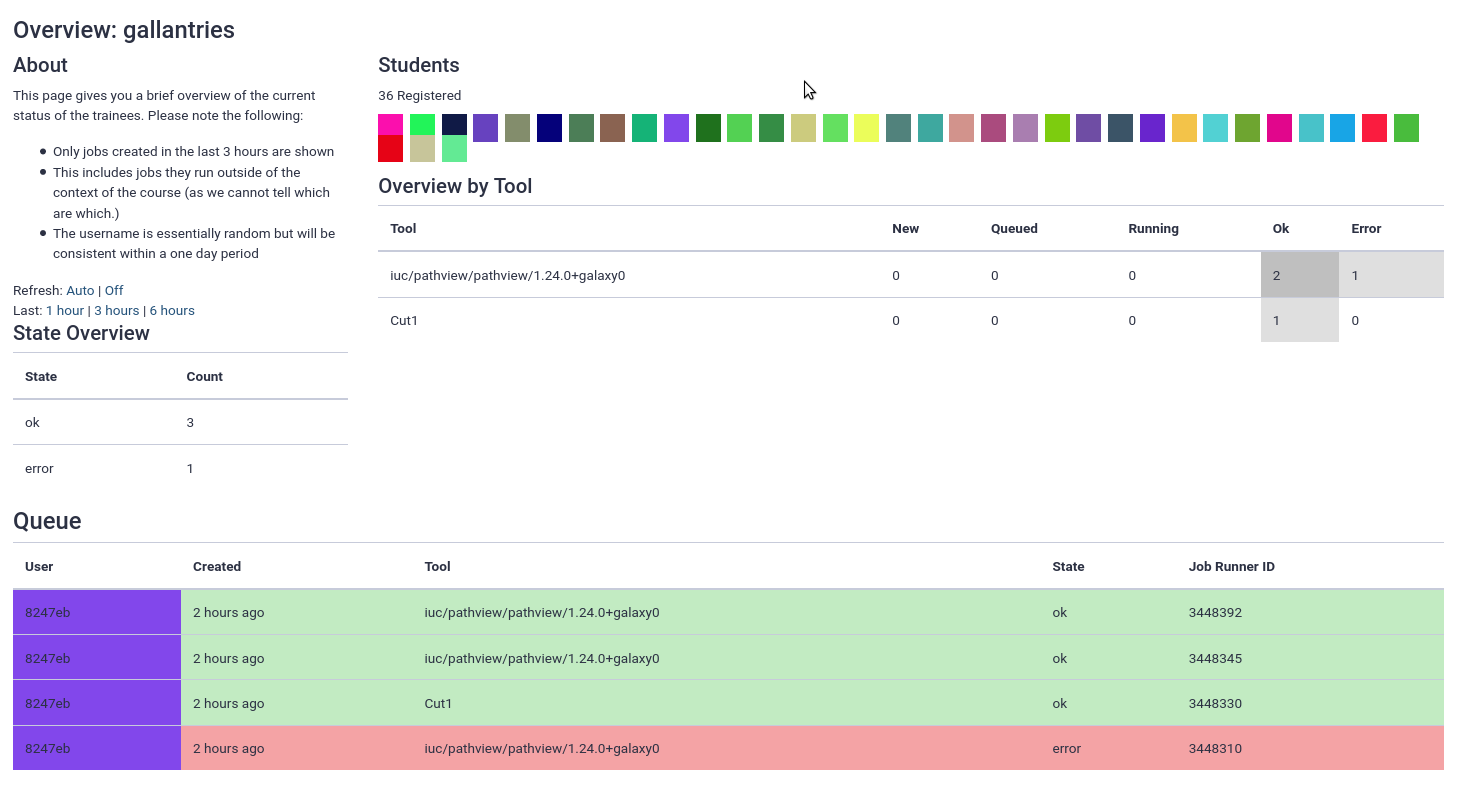
\includegraphics[width=0.8\textwidth]{images/tiaas.png}
	\caption{The dashboard provides anonymised observability into class progress, trainers can see at a glance if everyone has completed the quality control steps, or if there are any errors that they should ask the students to raise with the class.\label{fig:tiaas}}
\end{figure}

\begin{figure}[!ht]
	\centering
	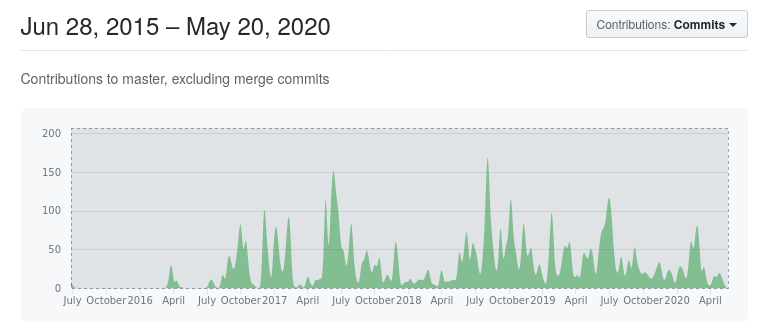
\includegraphics[width=0.8\textwidth]{images/commits.png}
	\caption{Graph of contributions to the training materials repository\label{fig:contributions}}
\end{figure}

\begin{figure}[!ht]
	\centering
	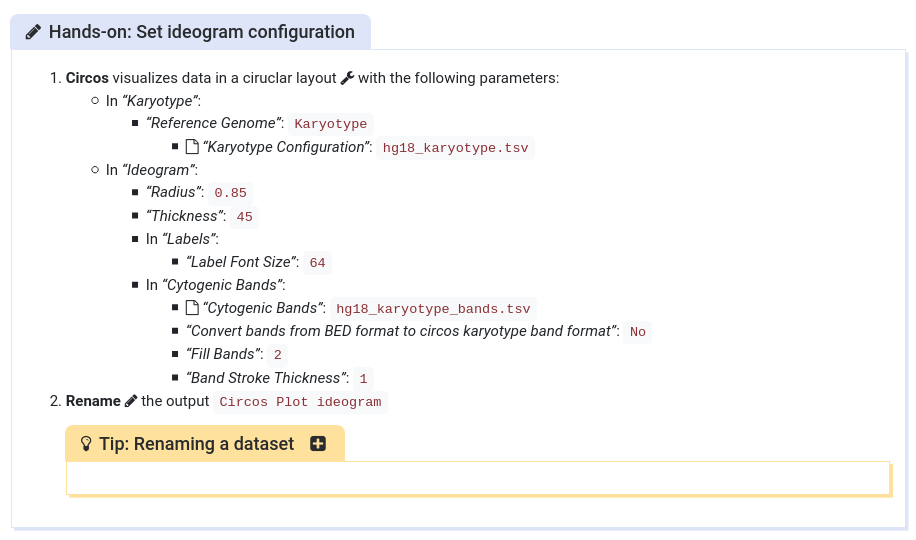
\includegraphics[width=0.8\textwidth]{images/tool-in-tutorial.png}
	\caption{Here we show an automatically generated snippet box, all of the relevant parameters have been extracted from the workflow. Where parameters are left to their default values, they are not mentioned. Where they are changed, detained instructions about the precise parameters and their names are documented.\label{fig:planemo}}
\end{figure}

\section*{Supporting information}

% Include only the SI item label in the paragraph heading. Use the \nameref{label} command to cite SI items in the text.
\paragraph*{S1 Fig.}
\label{S1_Fig}
{\bf Bold the title sentence.} Add descriptive text after the title of the item (optional).

\paragraph*{S2 Fig.}
\label{S2_Fig}
{\bf Lorem ipsum.} Maecenas convallis mauris sit amet sem ultrices gravida. Etiam eget sapien nibh. Sed ac ipsum eget enim egestas ullamcorper nec euismod ligula. Curabitur fringilla pulvinar lectus consectetur pellentesque.

\paragraph*{S1 File.}
\label{S1_File}
{\bf Lorem ipsum.}  Maecenas convallis mauris sit amet sem ultrices gravida. Etiam eget sapien nibh. Sed ac ipsum eget enim egestas ullamcorper nec euismod ligula. Curabitur fringilla pulvinar lectus consectetur pellentesque.

\paragraph*{S1 Video.}
\label{S1_Video}
{\bf Lorem ipsum.}  Maecenas convallis mauris sit amet sem ultrices gravida. Etiam eget sapien nibh. Sed ac ipsum eget enim egestas ullamcorper nec euismod ligula. Curabitur fringilla pulvinar lectus consectetur pellentesque.

\paragraph*{S1 Appendix.}
\label{S1_Appendix}
{\bf Lorem ipsum.} Maecenas convallis mauris sit amet sem ultrices gravida. Etiam eget sapien nibh. Sed ac ipsum eget enim egestas ullamcorper nec euismod ligula. Curabitur fringilla pulvinar lectus consectetur pellentesque.

\paragraph*{S1 Table.}
\label{S1_Table}
\begin{table}[]
\begin{adjustwidth}{-2.25in}{0in} % Comment out/remove adjustwidth environment if table fits in text column.
	\centering
	\caption{Top 10 tutorials in terms of visited pages given the Google Analytics stats. Table extracted using \href{https://github.com/bebatut/galaxy-training-material-stats/blob/master/src/extract_repo_content_stats.ipynb}{Jupyter Notebook} on 2019-04-12.\label{tbl:topViewedTutorials}}
	\begin{tabular}{ll}
		Tutorial                                                             & Average number of visits per month \\\hline
		Reference-based RNA-Seq data analysis (Transcriptomics)              & 1763 \\
		16S Microbial Analysis with mothur (Metagenomics)                    & 1418 \\
		Visualization of RNA-Seq results with Volcano Plot (Transcriptomics) & 1299 \\
		Quality Control (Sequence analysis)                                  & 1170 \\
		Galaxy 101 (Introduction)                                            & 768 \\
		Mapping (Sequence analysis)                                          & 701 \\
		Visualization of RNA-Seq results with Heatmap (Transcriptomics)      & 686 \\
		Genome annotation                                                    & 585 \\
		RNA-Seq reads to counts (Transcriptomics)                            & 575 \\
		General tutorial (Metagenomics)                                      & 500 \\
	\end{tabular}
\end{adjustwidth}
\end{table}

\paragraph*{S2 Table.}
\label{S2_Table}
\begin{table}[]
\begin{adjustwidth}{-2.25in}{0in} % Comment out/remove adjustwidth environment if table fits in text column.
	\centering
	\caption{Top 10 tutorials by number of Pull Request on the GitHub repository. Table extracted using \href{https://github.com/bebatut/galaxy-training-material-stats/blob/master/src/extract_repo_content_stats.ipynb}{Jupyter Notebook} on 2019-04-12.\label{tbl:topEditedTutorials}}
	\begin{tabular}{l|lll}
		Tutorials                           & Creation   & Number of Pull Requests & Mean duration between PRs\\\hline
		Reference-based RNA-seq             & 2016-10-05 & 78                      & 16 days\\
		16S Microbial Analysis with mothur  & 2017-02-12 & 55                      & 18 days\\
		Mapping                             & 2016-10-04 & 50                      & 22 days\\
		Quality control                     & 2016-10-04 & 45                      & 27 days\\
		De novo transcriptomics             & 2017-02-19 & 45                      & 20 days\\
		From peaks to genes                 & 2017-05-24 & 44                      & 15 days\\
		DNA Methylation data analysis       & 2016-10-05 & 42                      & 22 days\\
		De novo RAD seq                     & 2017-02-14 & 42                      & 28 days\\
		Reference-based RAD-seq             & 2017-02-14 & 40                      & 31 days\\
		Calling variants in diploid systems & 2016-08-19 & 40                      & 28 days\\
	\end{tabular}
\end{adjustwidth}
\end{table}


\paragraph*{S3 Table.}
\label{S3_Table}
\begin{table}[]
\begin{adjustwidth}{-2.25in}{0in} % Comment out/remove adjustwidth environment if table fits in text column.
	\centering
	\caption{Statistics about Pull Request on GitHub repository.\label{tbl:pullRequestReviewing}}
	\begin{tabular}{l|p{0.2\textwidth}p{0.2\textwidth}p{0.2\textwidth}p{0.2\textwidth}}
									        & Number & Reviews and comments (mean number per PR) & Reviewers (mean number per PR) & Duration (mean per PR) \\\hline
		Pull Requests to add tutorial(s)    & 135    & 9.3                                       & 2.7                            & 26 days\\
		Pull Requests to update tutorial(s) & 683    & 3.4                                       & 1.7                            & 11 days\\
		Other Pull Requests                 & 386    & 2.5                                       & 1.5                            & 5 days\\
	\end{tabular}
\end{adjustwidth}
\end{table}



\begin{table}[]
\begin{adjustwidth}{-2.25in}{0in} % Comment out/remove adjustwidth environment if table fits in text column.
	\centering
	\caption{Numbers of tutorials, slides, hands-on tutorials and other material per topics. \label{tbl:numberOfMaterials}}
	\begin{tabular}{p{2in}|p{0.8in}llp{0.8in}lll}
		Topics                                       & Introduction slide decks & Tutorials & Slide decks & Hands-on tutorials & Workflows & Data on Zenodo & Data on data library\\\hline
		Introduction to Galaxy Analyses              & 1                        & 8         & 1           & 7                  & 3         & 7              & 3\\
		Assembly                                     & 0                        & 4         & 3           & 4                  & 4         & 4              & 4\\
		Computational chemistry                      & 0                        & 4         & 0           & 4                  & 3         & 4              & 0\\
		Ecology                                      & 0                        & 5         & 0           & 5                  & 4         & 4              & 4\\
		Epigenetics                                  & 2                        & 5         & 2           & 5                  & 5         & 5              & 4\\
		Genome Annotation                            & 1                        & 4         & 2           & 4                  & 2         & 4              & 4\\
		Imaging                                      & 0                        & 2         & 0           & 2                  & 2         & 2              & 2\\
		Metabolomics                                 & 1                        & 3         & 0           & 3                  & 3         & 3              & 2\\
		Metagenomics                                 & 1                        & 5         & 0           & 5                  & 5         & 5              & 4\\
		Proteomics                                   & 0                        & 14        & 0           & 14                 & 13        & 14             & 9\\
		Sequence analysis                            & 0                        & 2         & 2           & 2                  & 2         & 2              & 2\\
		Statistics and machine learning              & 0                        & 4         & 0           & 4                  & 4         & 4              & 4\\
		Transcriptomics                              & 1                        & 19        & 3           & 18                 & 16        & 18             & 13\\
		Variant Analysis                             & 1                        & 6         & 0           & 6                  & 4         & 6              & 6\\
		Data Manipulation                            &                          & 7         & 1           & 6                  &           & 6              & \\
		User Interface and Features                  &                          & 4         & 0           & 4                  & 1         & 4              & 1\\
		Development in Galaxy                        & 1                        & 13        & 12          & 4                  &           &                & \\
		Galaxy Server administration                 & 1                        & 31        & 24          & 16                 &           & 6              & \\
		Contributing to the Galaxy Training Material & 1                        & 10        & 2           & 9                  &           &                & \\
		Teaching and Hosting Galaxy training         & 0                        & 5         & 1           & 4                  &           &                & \\
	\end{tabular}
\end{adjustwidth}
\end{table}


\section*{Acknowledgments}
Cras egestas velit mauris, eu mollis turpis pellentesque sit amet. Interdum et malesuada fames ac ante ipsum primis in faucibus. Nam id pretium nisi. Sed ac quam id nisi malesuada congue. Sed interdum aliquet augue, at pellentesque quam rhoncus vitae.

%\nolinenumbers


% Either type in your references using
% \begin{thebibliography}{}
% \bibitem{}
% Text
% \end{thebibliography}
%
% or
%
% Compile your BiBTeX database using our plos2015.bst
% style file and paste the contents of your .bbl file
% here. See http://journals.plos.org/plosone/s/latex for
% step-by-step instructions.
%

\bibliography{references}

%\begin{thebibliography}{10}

%\bibitem{bib1}
%Conant GC, Wolfe KH.
%\newblock {{T}urning a hobby into a job: how duplicated genes find new
  %functions}.
%\newblock Nat Rev Genet. 2008 Dec;9(12):938--950.

%\bibitem{bib2}
%Ohno S.
%\newblock Evolution by gene duplication.
%\newblock London: George Alien \& Unwin Ltd. Berlin, Heidelberg and New York:
  %Springer-Verlag.; 1970.

%\bibitem{bib3}
%Magwire MM, Bayer F, Webster CL, Cao C, Jiggins FM.
%\newblock {{S}uccessive increases in the resistance of {D}rosophila to viral
  %infection through a transposon insertion followed by a {D}uplication}.
%\newblock PLoS Genet. 2011 Oct;7(10):e1002337.

%\end{thebibliography}



\end{document}

